\chapter{Data analysis and results}
In this chapter we will describe approaches we used for analysis of binary matrix created in previous chapter. 
Firstly, we will visualize data to get basic idea about how closely related these data are and how much variance they represent.
Next, we will describe method used for selecting important characteristics.
We will also explain how we generated our predictive models and we will reveal how we evaluated them.

\section{Principal component analysis}
Principal component analysis (PCA) is method mostly used for visualization of high dimensional data.
For matrix with $r$ rows and $c$ columns it creates $min(r-1, c)$ distinct principal components.
Principal components are linearly uncorrelated variables created in such way that first principal component preserves most variance from original dataset, with each subsequent principal component preserving less than previous one.

For principal component analysis we used python library scikit-learn \cite{sklearn}.
Binary matrix was used as input.
First few principal components were used to create plots in python library matplotlib.
In the Figure (\ref{pca}) we can see data visualized with principal component one on the x-axis and principal component two on the y-axis.
Each data point represents one phage record and the color of particular data point corresponds to genus of that phage.
As we can see, most phage records are located near point $[0, 0]$, with some clear groups of Mycobacterium and Staphylococcus phages outside the center.
Although, this could suggest difficulties with distinguishing different genera, it was not the case as first two principal components retained less than 15\% of dataset variability.
Therefore, we proceeded with another analysis method.

\begin{figure}[htp]
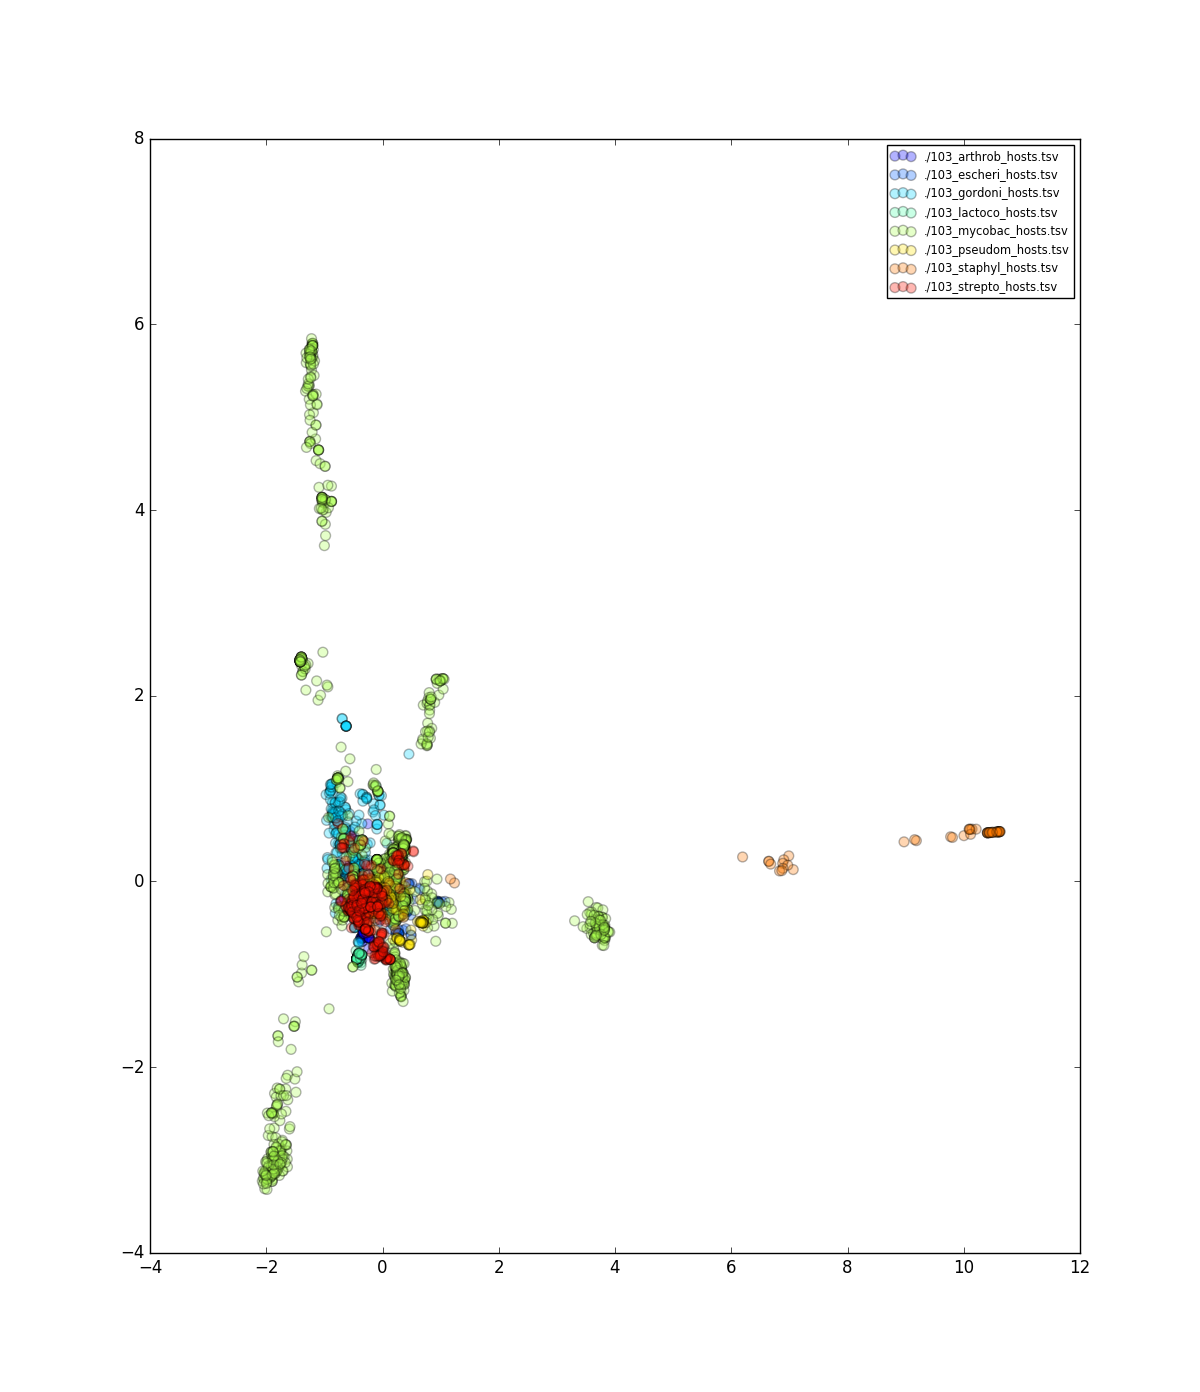
\includegraphics[width=\linewidth]{./images/pca.png}
\centering
\caption{PCA - first two principal components}
\end{figure}

\section{Decision tree}
Decision tree is a model, which we can imagine as binary tree.
In this tree, every node is either decision node or end node.
Decision node contains condition and has two child nodes.
First child node represents all cases, where the condition was not met and the second child node represents all cases, where condition was met.
These child nodes can be another decision node or end node.
End nodes do not contain any conditions and they represent the final decision made by model.

Decision tree is the simplest predictive model and contains exclusively conditions.
Usually, we need two sets of data to create the model, commonly called features and labels.
Features represent data which are known before prediction and labels represent expected results of prediction.
For example, features could be size, weight, length of nose and color and labels could be if animal described by those features is a dog or if it is a cat.

Decision tree model has advantages, which led us to conclusion it will suit our needs.
Namely, these are the option to easily visualize the model, interpret the results, availability in many programming libraries and its good documentation.
The fact that decision tree model is a white box model allowed us to extract further information from our models, for example importance of particular clusters for predictions.

Of course, there are also disadvantages of this model.
One of the biggest disadvantage is, decision tree model is prone to overfitting of data.
It means that sometimes the resulting model does not generalize the data well enough and the accuracy of real predictions can be lowered.
Another disadvantage is, the models are often biased when predicting multiple classes with unbalanced dataset.
These issues was addressed with methods mentioned further.

\section{Feature selection}
Up to now, our training dataset consisted of matrix with 2787 rows, representing phages and 15017 columns, representing gene clusters.
This high dimensionality of our data could lead to increased probability of overfitting of models on data.
To address this concern, we decided to perform feature selection.
Feature selection is a process of removing dimensions with low importance from the dataset.
The reason to prefer feature selection over feature extraction methods as PCA presented in previous section was, we wanted our tree models to be representable in terms of important clusters rather than in terms of principal components.
Because we expected a lot of clusters with small number of genes, our choice for feature selection method was Variance Threshold.
The Variance Threshold method is a simple method, which removes columns with variance under certain threshold.
With this technique we removed all columns in matrix with ones in more than 99\% of cases or with zeros in more than 99\% of cases.
The reduced matrix had 2787 rows and 1818 columns.

\section{Building decision tree models}
In our work we used Decision Tree Classifier from python library scikit-learn.
For each group of phages with hosts from eight selected genera we created one model.
Each of those models was trained to answer question, if one particular phage was able to infect bacteria from particular genus.
For example, for created model Mycobacterium we could ask if given phage sequence is able to infect bacteria from Mycobacterium genus.
The model will return one or zero, where one represents that model assumes that the given sequence belong to Mycobacterium phage and zero represents that model assumes it does not belong to Mycobacterium phage.
Models were trained with reduced matrix used as features.
The ability to infect particular genus was used as labels.
We marked this as one if the particular phage was able to infect particular host and zero otherwise.
To prevent overfitting of our trees, we also used parameter \verb|min_impurity_split=0.03|.
This enabled threshold for splitting leaves and therefore only nodes with impurity index greater than 0.03 were divided.
The threshold 0.03 was determined empirically.
Lower values created tree with many nodes, where the risk of overfitting was high and greater values did not have enough nodes to maintain models accuracy.
With this approach we created model for each of our eight selected host genera and visualized it with python library graphviz.
We can see example of this visualization in the Figure \ref{fig:tree}.

\begin{figure}[htp]
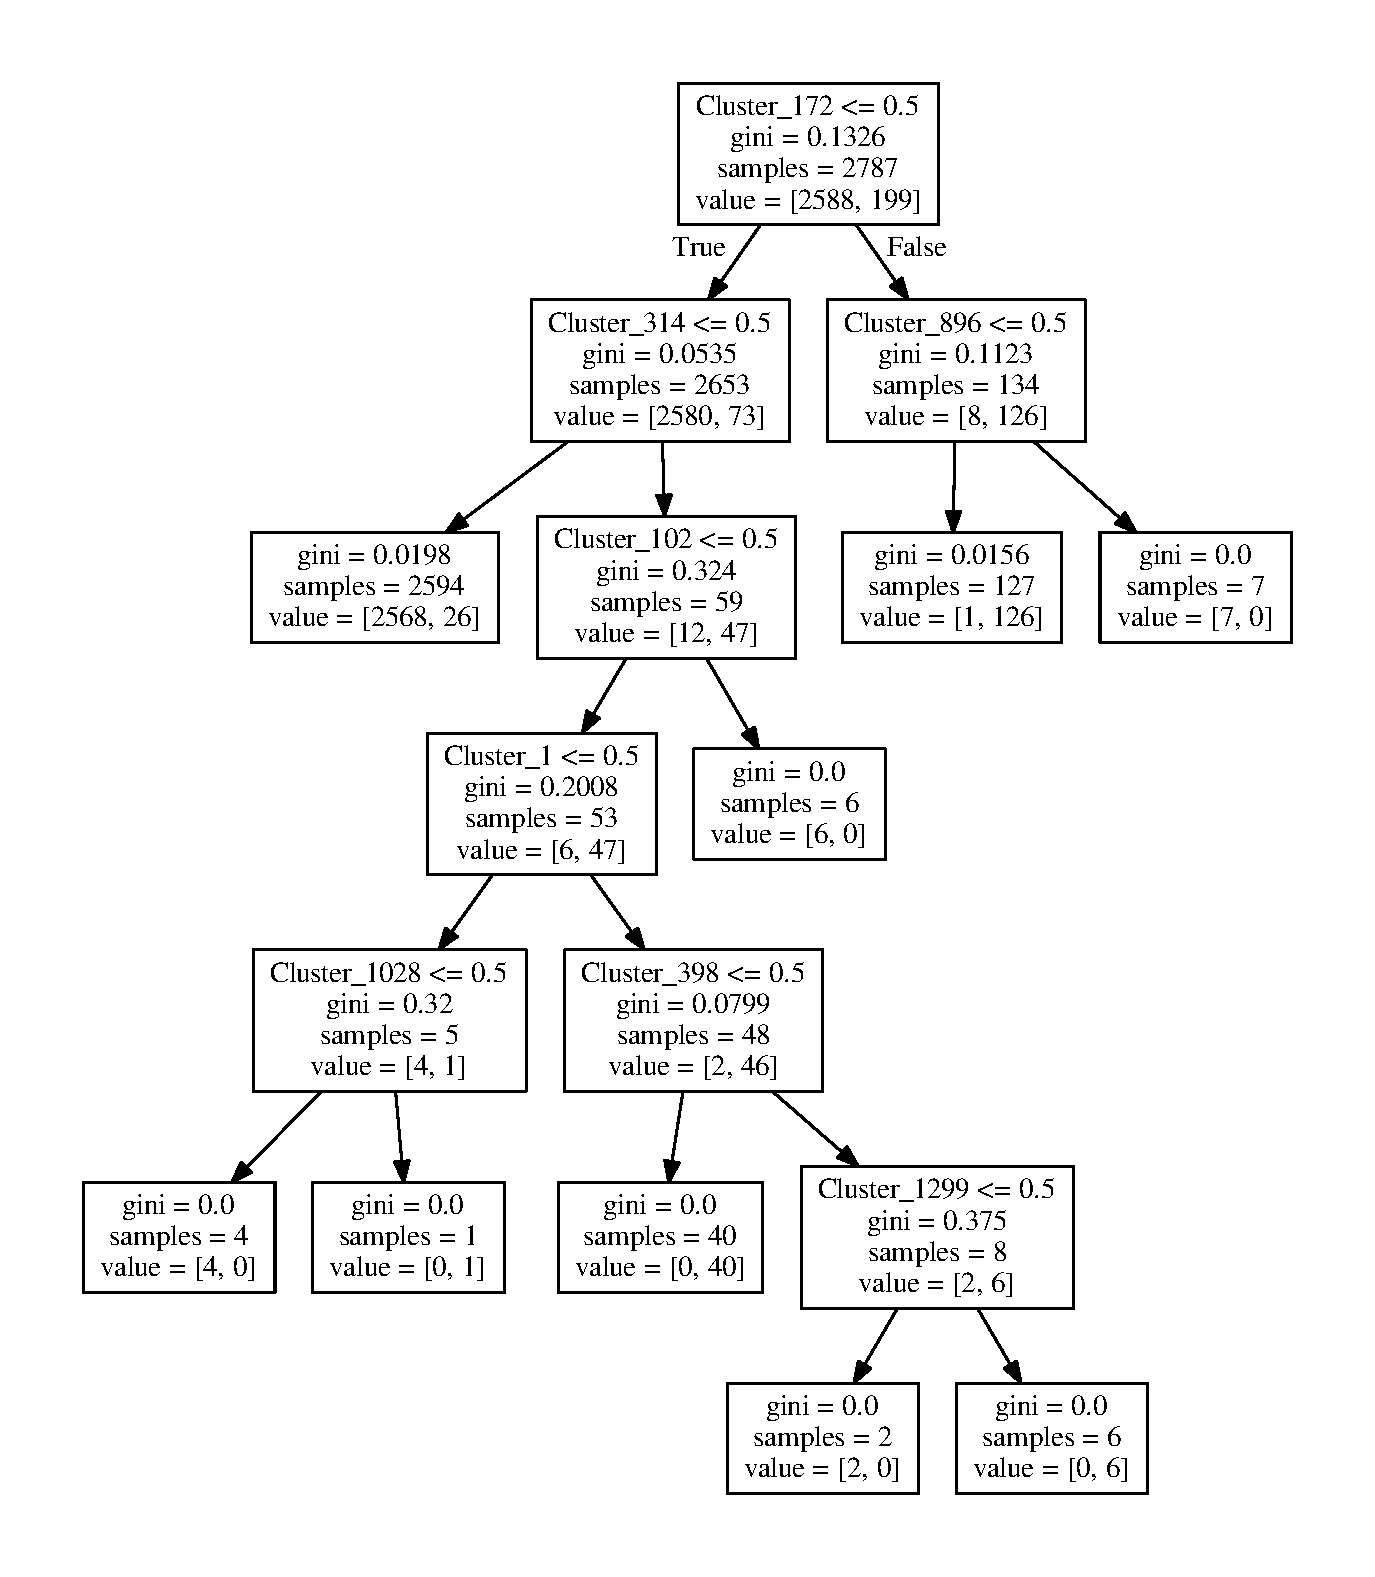
\includegraphics[width=\linewidth]{./images/tree.pdf}
\centering
\caption{Arthrobacter model}
\label{fig:tree}
\end{figure}

From the Figure we can see that cluster number 172 provides the best division of phages infecting Arthrobacter genus.
Most Arthrobacter phages have some gene from this cluster.
This suggests genes from this cluster are of high importance for Arthrobacter phages and could participate on important mechanism for infecting bacteria from genus Arthrobacter.
Of course, these claims need to be supported by additional evidence and biological experiments, but it can provide valuable insight into data.
We can analyze other graph nodes similarly.
Finally, the models were stored using python library pickle for later use.

% http://scikit-learn.org/stable/modules/tree.html

\section{Classification from sequence}
For classification we expected to have complete sequence of bacteriophage.
This sequence was annotated using Prokka and genes were extracted using custom script.
Extracted genes were aligned using BLAST to database of genes from training set.
We assigned cluster number to all newly obtained genes based on the cluster number of the most similar gene from BLAST database.
Thereafter, vector of ones and zeros was created for each phage representing if phage contains gene from particular cluster - similar to new row in matrix.
This vector was passed to decision tree model and resulting prediction was saved.

\section{Evaluation of models}
To examine accuracy of our models, we classified all bacteriophages from our test dataset.
Test dataset contained 699 phage records.
Resulting predictions were aggregated and number of correctly predicted, false positive and false negative was recorded.
The table was constructed from these data.
Accuracy was calculated as $CP/(CP+FP+FN)$, false positive percentage as $FP/(CP+FP+FN)$ and false negative percentage as $FN/(CP+FP+FN)$.
We can see summary of model statistics in the Table \ref{tab:models}. 

\begin{table}
  \centering
    \begin{tabular}{ r l l l l l l }
	\hline
	model & correct & fpos & fneg & accuracy & fposp & fnegp \\
	\hline
	Arthrobacter & 683 & 11 & 5  & 97.71\% & 1.57\% & 0.71\% \\
	Escherichia & 679 & 17 & 3  & 97.13\% & 2.43\% & 0.42\% \\
	Gordonia & 647 & 39 & 13 & 92.56\% & 5.57\% & 1.85\% \\
	Lactococcus & 680 & 3  & 16 & 97.28\% & 0.42\% & 2.28\% \\
	Mycobacterium & 686 & 11 & 2  & 98.14\% & 1.57\% & 0.28\% \\
	Pseudomonas & 686 & 6  & 7  & 98.14\% & 0.85\% & 1.00\% \\
	Staphylococcus & 685 & 0  & 14 & 97.99\% & 0.00\% & 2.00\% \\
	Streptococcus & 686 & 2  & 11 & 98.14\% & 0.28\% & 1.57\% \\
	\end{tabular}
	\bigskip
    \caption{Evaluation of models}
    \label{tab:models}
\end{table}

\section{Limitations and future work}
Although high accuracy of our predictions, we are aware of potential improvement in the future.
Sequences used were mostly annotated only with one host. 
Despite high phage specificity, some phages can have multiple hosts.
One of the goal to the future will be to collect more accurate dataset with experimentally confirmed non-hosts.
Also, relatively small number of phages are known to mankind, despite of approximately 200 newly discovered phages appears in databases every month. 
With greater and more accurate dataset we would be able to create models to the taxonomical levels of species or even strains.
For the future we would also like to try this method for predicting from incomplete sequences, as this will be mostly the case in practice.
This could lead to novel methods for indirect diagnosis of microbiome.

%In the future we will also experiment with different clustering methods and different machine learning approaches. 
% better datasets
% better clustering algorithms
% not sure if it is possible to classify from incomplete sequences
% inability to discover phages with brand new mechanism
% decreased accuracy in insufficiently discovered phage genera